\documentclass[
	% -- opções da classe memoir --
	12pt,				% tamanho da fonte
	openright,			% capítulos começam em pág ímpar (insere página vazia caso preciso)
	twoside,			% para impressão em recto e verso. Oposto a oneside
	a4paper,			% tamanho do papel. 
	% -- opções da classe abntex2 --
	%chapter=TITLE,		% títulos de capítulos convertidos em letras maiúsculas
	%section=TITLE,		% títulos de seções convertidos em letras maiúsculas
	%subsection=TITLE,	% títulos de subseções convertidos em letras maiúsculas
	%subsubsection=TITLE,% títulos de subsubseções convertidos em letras maiúsculas
	% -- opções do pacote babel --
	english,			% idioma adicional para hifenização
	brazil				% o último idioma é o principal do documento
	]{abntex2}

% ---
% Pacotes básicos 
% ---
\usepackage{lmodern}			% Usa a fonte Latin Modern			
\usepackage[T1]{fontenc}		% Selecao de codigos de fonte.
\usepackage[utf8]{inputenc}		% Codificacao do documento (conversão automática dos acentos)
\usepackage{lastpage}			% Usado pela Ficha catalográfica
\usepackage{indentfirst}		% Indenta o primeiro parágrafo de cada seção.
\usepackage{color}				% Controle das cores
\usepackage{graphicx}			% Inclusão de gráficos
\graphicspath{{imagens/}}
\usepackage{microtype} 			% para melhorias de justificação
\usepackage{amsmath}
\usepackage{caption} 
\usepackage{multirow}
\usepackage{subfig}

% ---
		
% ---
% Pacotes adicionais, usados apenas no âmbito do Modelo Canônico do abnteX2
% ---
\usepackage{lipsum}				% para geração de dummy text
% ---

% ---
% Pacotes de citações
% ---
\usepackage[brazilian,hyperpageref]{backref}	 % Paginas com as citações na bibl
\usepackage[alf]{abntex2cite}	% Citações padrão ABNT

% --- 
% CONFIGURAÇÕES DE PACOTES
% --- 

% ---
% Configurações do pacote backref
% Usado sem a opção hyperpageref de backref
\renewcommand{\backrefpagesname}{Citado na(s) página(s):~}
% Texto padrão antes do número das páginas
\renewcommand{\backref}{}
% Define os textos da citação
\renewcommand*{\backrefalt}[4]{
	\ifcase #1 %
		Nenhuma citação no texto.%
	\or
		Citado na página #2.%
	\else
		Citado #1 vezes nas páginas #2.%
	\fi}%
% ---

% ---
% Informações de dados para CAPA e FOLHA DE ROSTO
% ---
\titulo{Análise do estudo 320 do \textit{AIDS Clinical Trials Group}}
\autor{Augusto Cesar Ribeiro Nunes - 13/0103004 \\
	Isabela Paranhos Pinto - 11/0013450}
\local{Distrito Federal, Brasil}
\data{Dezembro de 2016}
% \orientador{Lauro César Araujo}
% \coorientador{Equipe \abnTeX}
\instituicao{%
  Universidade de Brasília
  \par
  Instituto de Ciências Exatas
  \par
  Departamento de Estatística
  \par
  Graduação}
\tipotrabalho{Trabalho Final de Disciplina (Graduação)}
% O preambulo deve conter o tipo do trabalho, o objetivo, 
% o nome da instituição e a área de concentração 
\preambulo{Trabalho final da disciplina Análise de Sobrevivência, ministrada pela Profa. Dra. Juliana Betini Fachini Gomes ao curso de bacharelado em Estatística da Universidade de Brasília, no segundo semestre de 2016}
% ---


% ---
% Configurações de aparência do PDF final

% alterando o aspecto da cor azul
\definecolor{blue}{RGB}{41,5,195}

% informações do PDF
\makeatletter
\hypersetup{
     	%pagebackref=true,
		pdftitle={\@title}, 
		pdfauthor={\@author},
    	pdfsubject={\imprimirpreambulo},
	    pdfcreator={LaTeX with abnTeX2},
		pdfkeywords={abnt}{latex}{abntex}{abntex2}{trabalho acadêmico}, 
		colorlinks=true,       		% false: boxed links; true: colored links
    	linkcolor=blue,          	% color of internal links
    	citecolor=blue,        		% color of links to bibliography
    	filecolor=magenta,      		% color of file links
		urlcolor=blue,
		bookmarksdepth=4
}
\makeatother
% --- 

% --- 
% Espaçamentos entre linhas e parágrafos 
% --- 

% O tamanho do parágrafo é dado por:
\setlength{\parindent}{1.3cm}

% Controle do espaçamento entre um parágrafo e outro:
\setlength{\parskip}{0.2cm}  % tente também \onelineskip

% ---
% compila o indice
% ---
\makeindex
% ---

% ----
% Início do documento
% ----
\begin{document}

% Seleciona o idioma do documento (conforme pacotes do babel)
%\selectlanguage{english}
\selectlanguage{brazil}

% Retira espaço extra obsoleto entre as frases.
\frenchspacing 

% ----------------------------------------------------------
% ELEMENTOS PRÉ-TEXTUAIS
% ----------------------------------------------------------
% \pretextual

% ---
% Capa
% ---
\imprimircapa
% ---

% ---
% Folha de rosto
% (o * indica que haverá a ficha bibliográfica)
% ---
\imprimirfolhaderosto*
% ---

% ---
% Inserir a ficha bibliografica
% ---

% Isto é um exemplo de Ficha Catalográfica, ou ``Dados internacionais de
% catalogação-na-publicação''. Você pode utilizar este modelo como referência. 
% Porém, provavelmente a biblioteca da sua universidade lhe fornecerá um PDF
% com a ficha catalográfica definitiva após a defesa do trabalho. Quando estiver
% com o documento, salve-o como PDF no diretório do seu projeto e substitua todo
% o conteúdo de implementação deste arquivo pelo comando abaixo:
%
% \begin{fichacatalografica}
%     \includepdf{fig_ficha_catalografica.pdf}
% \end{fichacatalografica}

% \begin{fichacatalografica}
% 	\sffamily
% 	\vspace*{\fill}					% Posição vertical
% 	\begin{center}					% Minipage Centralizado
% 	\fbox{\begin{minipage}[c][8cm]{13.5cm}		% Largura
% 	\small
% 	\imprimirautor
% 	%Sobrenome, Nome do autor
	
% 	\hspace{0.5cm} \imprimirtitulo  / \imprimirautor. --
% 	\imprimirlocal, \imprimirdata-
	
% 	\hspace{0.5cm} \pageref{LastPage} p. : il. (algumas color.) ; 30 cm.\\
	
% 	\hspace{0.5cm} \imprimirorientadorRotulo~\imprimirorientador\\
	
% 	\hspace{0.5cm}
% 	\parbox[t]{\textwidth}{\imprimirtipotrabalho~--~\imprimirinstituicao,
% 	\imprimirdata.}\\
	
% 	\hspace{0.5cm}
% 		1. Trabalho Final de Disciplina.
% 		2. Análise de Sobrevivência.
% 		2. Palavra-chave3.
% 		I. Juliana Betini Fachini Gomes.
% 		II. Universidade de Brasília.
% 		III. Departamento de Estatística.
% 		IV. Análise do estudo 320 do \textit{AIDS Clinical Trials Group} 			
% 	\end{minipage}}
% 	\end{center}
% \end{fichacatalografica}
% ---

% ---
% Inserir errata
% ---
% \begin{errata}
% Elemento opcional da \citeonline[4.2.1.2]{NBR14724:2011}. Exemplo:

% \vspace{\onelineskip}

% FERRIGNO, C. R. A. \textbf{Tratamento de neoplasias ósseas apendiculares com
% reimplantação de enxerto ósseo autólogo autoclavado associado ao plasma
% rico em plaquetas}: estudo crítico na cirurgia de preservação de membro em
% cães. 2011. 128 f. Tese (Livre-Docência) - Faculdade de Medicina Veterinária e
% Zootecnia, Universidade de São Paulo, São Paulo, 2011.

% \begin{table}[htb]
% \center
% \footnotesize
% \begin{tabular}{|p{1.4cm}|p{1cm}|p{3cm}|p{3cm}|}
%   \hline
%    \textbf{Folha} & \textbf{Linha}  & \textbf{Onde se lê}  & \textbf{Leia-se}  \\
%     \hline
%     1 & 10 & auto-conclavo & autoconclavo\\
%    \hline
% \end{tabular}
% \end{table}

% \end{errata}
% ---

% ---
% Inserir folha de aprovação
% ---

% Isto é um exemplo de Folha de aprovação, elemento obrigatório da NBR
% 14724/2011 (seção 4.2.1.3). Você pode utilizar este modelo até a aprovação
% do trabalho. Após isso, substitua todo o conteúdo deste arquivo por uma
% imagem da página assinada pela banca com o comando abaixo:
%
% \includepdf{folhadeaprovacao_final.pdf}
%
% \begin{folhadeaprovacao}

%   \begin{center}
%     {\ABNTEXchapterfont\large\imprimirautor}

%     \vspace*{\fill}\vspace*{\fill}
%     \begin{center}
%       \ABNTEXchapterfont\bfseries\Large\imprimirtitulo
%     \end{center}
%     \vspace*{\fill}
    
%     \hspace{.45\textwidth}
%     \begin{minipage}{.5\textwidth}
%         \imprimirpreambulo
%     \end{minipage}%
%     \vspace*{\fill}
%    \end{center}
        
%    Trabalho aprovado. \imprimirlocal, 24 de novembro de 2012:

%    \assinatura{\textbf{\imprimirorientador} \\ Orientador} 
%    \assinatura{\textbf{Professor} \\ Convidado 1}
%    \assinatura{\textbf{Professor} \\ Convidado 2}
%    %\assinatura{\textbf{Professor} \\ Convidado 3}
%    %\assinatura{\textbf{Professor} \\ Convidado 4}
      
%    \begin{center}
%     \vspace*{0.5cm}
%     {\large\imprimirlocal}
%     \par
%     {\large\imprimirdata}
%     \vspace*{1cm}
%   \end{center}
  
% \end{folhadeaprovacao}
% ---

% ---
% Dedicatória
% ---
% \begin{dedicatoria}
%    \vspace*{\fill}
%    \centering
%    \noindent
%    \textit{ Este trabalho é dedicado às crianças adultas que,\\
%    quando pequenas, sonharam em se tornar cientistas.} \vspace*{\fill}
% \end{dedicatoria}
% ---

% ---
% Agradecimentos
% ---
% \begin{agradecimentos}
% Os agradecimentos principais são direcionados à Gerald Weber, Miguel Frasson,
% Leslie H. Watter, Bruno Parente Lima, Flávio de Vasconcellos Corrêa, Otavio Real
% Salvador, Renato Machnievscz\footnote{Os nomes dos integrantes do primeiro
% projeto abn\TeX\ foram extraídos de
% \url{http://codigolivre.org.br/projects/abntex/}} e todos aqueles que
% contribuíram para que a produção de trabalhos acadêmicos conforme
% as normas ABNT com \LaTeX\ fosse possível.

% Agradecimentos especiais são direcionados ao Centro de Pesquisa em Arquitetura
% da Informação\footnote{\url{http://www.cpai.unb.br/}} da Universidade de
% Brasília (CPAI), ao grupo de usuários
% \emph{latex-br}\footnote{\url{http://groups.google.com/group/latex-br}} e aos
% novos voluntários do grupo
% \emph{\abnTeX}\footnote{\url{http://groups.google.com/group/abntex2} e
% \url{http://www.abntex.net.br/}}~que contribuíram e que ainda
% contribuirão para a evolução do \abnTeX.

% \end{agradecimentos}
% ---

% ---
% Epígrafe
% ---
% \begin{epigrafe}
%     \vspace*{\fill}
% 	\begin{flushright}
% 		\textit{``Não vos amoldeis às estruturas deste mundo, \\
% 		mas transformai-vos pela renovação da mente, \\
% 		a fim de distinguir qual é a vontade de Deus: \\
% 		o que é bom, o que Lhe é agradável, o que é perfeito.\\
% 		(Bíblia Sagrada, Romanos 12, 2)}
% 	\end{flushright}
% \end{epigrafe}
% ---

% ---
% RESUMOS
% ---

% resumo em português
\setlength{\absparsep}{18pt} % ajusta o espaçamento dos parágrafos do resumo
\begin{resumo}
Esta análise do estudo número 320 do \textit{AIDS Clinical Trials Group}...

 \textbf{Palavras-chave}: Análise de Sobrevivência. abntex. editoração de texto.
\end{resumo}

% resumo em inglês
% \begin{resumo}[Abstract]
%  \begin{otherlanguage*}{english}
%    This is the english abstract.

%    \vspace{\onelineskip}
 
%    \noindent 
%    \textbf{Keywords}: latex. abntex. text editoration.
%  \end{otherlanguage*}
% \end{resumo}

% % resumo em francês 
% \begin{resumo}[Résumé]
%  \begin{otherlanguage*}{french}
%     Il s'agit d'un résumé en français.
 
%    \textbf{Mots-clés}: latex. abntex. publication de textes.
%  \end{otherlanguage*}
% \end{resumo}

% % resumo em espanhol
% \begin{resumo}[Resumen]
%  \begin{otherlanguage*}{spanish}
%    Este es el resumen en español.
  
%    \textbf{Palabras clave}: latex. abntex. publicación de textos.
%  \end{otherlanguage*}
% \end{resumo}
% ---

% ---
% inserir lista de ilustrações
% ---
% \pdfbookmark[0]{\listfigurename}{lof}
% \listoffigures*
% \cleardoublepage
% % ---

% % ---
% % inserir lista de tabelas
% % ---
% \pdfbookmark[0]{\listtablename}{lot}
% \listoftables*
% \cleardoublepage
% % ---

% % ---
% % inserir lista de abreviaturas e siglas
% % ---
% \begin{siglas}
%   \item[ABNT] Associação Brasileira de Normas Técnicas
%   \item[abnTeX] ABsurdas Normas para TeX
% \end{siglas}
% % ---

% % ---
% % inserir lista de símbolos
% % ---
% \begin{simbolos}
%   \item[$ \Gamma $] Letra grega Gama
%   \item[$ \Lambda $] Lambda
%   \item[$ \zeta $] Letra grega minúscula zeta
%   \item[$ \in $] Pertence
% \end{simbolos}
% ---

% ---
% inserir o sumario
% ---
\pdfbookmark[0]{\contentsname}{toc}
\tableofcontents*
\cleardoublepage
% ---



% ----------------------------------------------------------
% ELEMENTOS TEXTUAIS
% ----------------------------------------------------------
\textual

% ----------------------------------------------------------
% Introdução (exemplo de capítulo sem numeração, mas presente no Sumário)
% ----------------------------------------------------------
\chapter*[Introdução]{Introdução}
\addcontentsline{toc}{chapter}{Introdução}
% ----------------------------------------------------------
Este documento relata a análise do conjunto de dados produzido pelo estudo 320 do \textit{AIDS Clinical Trials Group} (ACTG). O ACTG é um grupo de trabalho multidisciplinar estabelecido em 1989 pela pesquisadora Maureen Myers do \textit{National Institutes of Health}. A Missão Institucional do grupo é "curar a infecção por HIV e reduzir o fardo das doenças devidas à infecção por HIV e suas complicações, incluindo tuberculose e hepatite viral".  

Na década de 80 os EUA foram o epicentro de uma epidemia de HIV que atingiu de maneira particularmente a população de homens que fazem sexo com homens (MSM) de três grandes centros urbanos do país: São Francisco, Nova Iorque e Los Angeles. As dificuldades de acesso a serviços de saúde e diagnóstico contribuíram para que a epidemia, que começou com cerca de 20 mil casos de infecção no período entre os anos de 1980-81, atingisse cerca de 130 mil novos casos diagnosticados no biênio 1984-5, conforme mostrado por \cite{el2010aids} e \cite{hall2008estimation}.

\cite{fauci2003hiv} mostra que atualmente existem 20 drogas aprovadas pelo \textit{Food and Drug Administration} nos EUA para o tratamento do HIV. O espectro de ação das drogas passa pelo tratamento da infecção primária e também a redução do risco de infecções secundárias, como Sarcoma de Kaposi e Turbeculose. Em razão da diversidade farmacológica destas drogas, em geral os pacientes diagnosticados recebem combinações destas 20 drogas, de acordo com seu perfil epidemiológico. Não é incomum que estas combinações mudem conforme o tratamento avança.

O número considerável de combinações e interações entre os medicamentos motiva estudos que analisam a resposta dos pacientes às diferentes formas de tratamento. Em \cite{hammer1997controlled}, foi realizado um estudo duplo-cego de Fase III\footnote{A Fase III de um estudo clínico é o último estágio de aprovação antes que um tratamento seja liberado.} que tinha como objetivo comparar a eficácia do tratamento combinado de Sulfato de Indinavir (IDV) em conjunto com Ziduvodina (ZDV/AZT) ou Estavudina (d4T) em conjunto com Lamivudina (3TC) em relação ao tratamento prévio com apenas Ziduvodina (ZDV) em 1156 pacientes com infecção por HIV cuja contagem de células CD4 era inferior a 200 células por $mm^3$ e tratamento prévio por ZDV superior a três meses. A ZDV foi o primeiro fármaco liberado para terapia antirretroviral nos EUA, em 1987; já o IDV foi liberado individualmente em março de 1996, cerca de um ano antes da publicação deste estudo. 

Os resultados mostraram que a nova terapia com os três medicamentos reduziu a proporção de pacientes soropositivos que evoluíram à AIDS ou morte quando comparada à terapia tradicional. Neste trabalho em particular o contexto é um pouco diferente: ao invés de considerarmos múltiplos eventos - AIDS ou morte - somente o falecimento do paciente é tratado como resposta. Esta adaptação altera sutilmente os achados do estudo, mas ainda sustenta como significativa a diferença entre os tratamentos.

Os resultados de Análise Exploratória são descritos no Capítulo \ref{chap:anexp}. O Modelo de Regressão é proposto em \ref{chap:modreg} e avaliado em \ref{chap:modav}. O conjunto de dados é descrito no Anexo \ref{anex:dados}.

Tradicionalmente, em cenários onde não estamos interessados necessariamente numa modelagem preditiva para o evento de interesse, utilizamos modelos semi-paramétricos - também conhecidos modelos de riscos proporcionais ou de Cox - para analisar os dados. Uma descrição do fenômeno completa do ponto de vista estatístico tem aqui interesse secundário e pode ser o caso que não seja sequer possível tal prescrição nos modelos paramétricos tradicionais, levando assim à proposição de novos modelos. Portanto, levando em consideração que este é um estudo de um tratamento em estágio final para disponibilização ao público, foi ajustado um modelo semi-paramétrico: nele temos interesse em caracterizar como a distribuição do evento de interesse muda de acordo com o comportamento das covariáveis, sua mudança sistemática. 

% ----------------------------------------------------------
% PARTE
% ----------------------------------------------------------
\part{Análise Exploratória}
% ----------------------------------------------------------
\chapter{Achados Exploratórios}
\label{chap:anexp}


\section{Medidas Descritivas para a variável tempo até a morte}
A Tabela \ref{tab:exp1} ilustra medidas descritivas para a variável tempo até a morte do paciente para os três grupos possíveis de censura: geral (censura ou falha), censurados e falha. A Figura \ref{fig:exp1} apresenta a densidade \textit{Kernel} para a variável em questão nos três grupos possíveis de censura. O comportamento muito similar da densidade do tempo em censura e do tempo geral sugere a ocorrência de poucas falhas - poucas mortes - no conjunto de dados. Tal comportamento pode ser justificado em termos do baixo tempo máximo observado, cerca de 1 ano (364 dias), ou também pelo fato do estudo ter sido interrompido por critério de parada baseado na eficácia demonstrada do novo tratamento durante as análises intermediárias.

\begin{table}[!ht]
	\caption{Medidas descritivas para a variável tempo até a morte do paciente}
    \label{tab:exp1}
    \centering
	\begin{tabular}{cccc}
    	\hline
		\multirow{2}{*}{Medida Descritiva} & \ &  Tempos (em dias) \\
        \ & Geral & Censurados & Falha \\\hline
        Mínimo & 1 & 1 & 15 \\
        $1^o$ Quartil & 194,5 & 201 & 81,25 \\
        Mediana & 265 & 121,5 & 266 \\
        Média & 242,2867 & 244,672 & 139,0769 \\
        $3^o$ Quartil & 306 & 203 & 307 \\
        Máximo & 364 & 287 & 364 \\\hline\hline
	\end{tabular}
    \caption*{\tiny{\textbf{Fonte}: Estudo 320 do \textit{AIDS Clinical Trials Group}}}
\end{table}

\begin{figure}[!ht]
	\centering
    \caption{Densidade \textit{Kernel} para a variável tempo}
    \label{fig:exp1}
	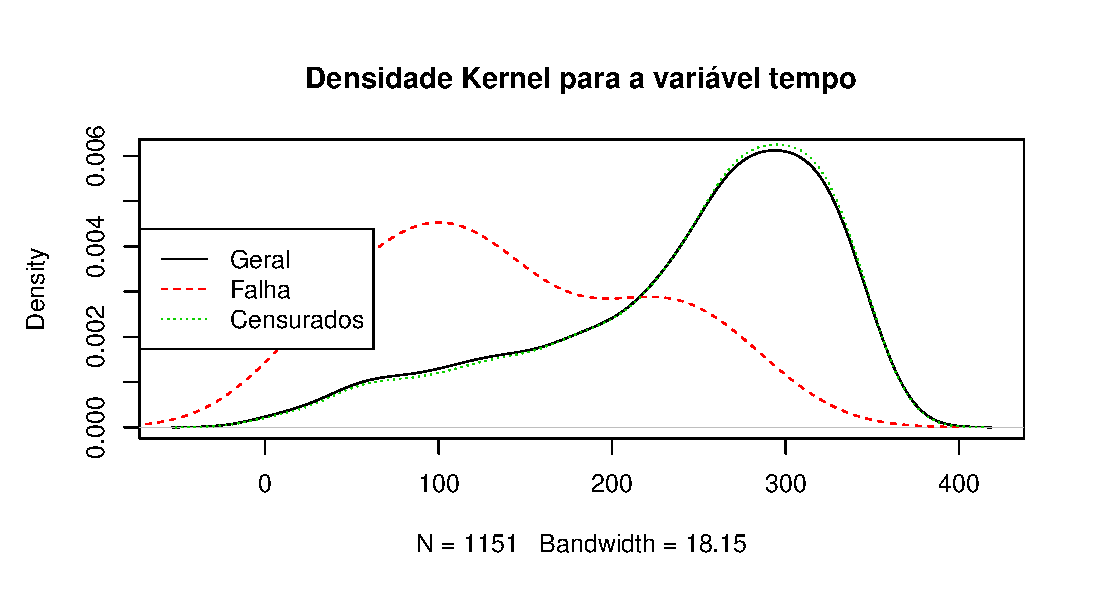
\includegraphics[scale = 0.9]{Rplot}
\end{figure}

A curva de sobrevivência estimada pelo Método de Kaplan-Meier sem considerar qualquer covariável está ilustrada na Figura \ref{fig:exp2}. Note como esta curva sugere a presença de uma função de sobrevivência imprópria, ou seja, temos $\hat{S}(t) \to k$, com $k \neq 0$. A utilização dos ditos Modelos de Fração de Cura, onde uma proporção de pacientes é considerada \textit{imune} à ocorrência do evento, modela bem este efeito. Há no entanto uma observação importante quanto à terminologia e sua aplicação no contexto de pacientes soropositivos para HIV: mesmo após 30 anos de pesquisas e avanços ainda não podemos falar plenamente em pacientes infectados e posteriormente \textit{curados} ou \textit{imunes}. Houve sim considerável avanço a ponto de garantir que os pacientes atinjam um nível satisfatório de qualidade de vida e, nesse sentido, possam nunca chegar a experimentar a falha (morte) decorrente da infecção primária por HIV, mas ainda assim precisamos ser reticentes quanto à terminologia. Vale reiterar que o estudo foi interrompido ao atingir um critério de eficácia durante uma avaliação preliminar, o que também pode reforçar as evidências no sentido da presença de fração de cura mesmo que epistemologicamente não seja o caso. Felizmente, dos 1156 pacientes observados no experimento, somente 26 - 2,25\% do total - observaram o evento.

\begin{figure}[!ht]
	\centering
    \caption{Estimativa segundo o Método de Kaplan-Meier para a curva de sobrevivência.}
    \label{fig:exp2}
    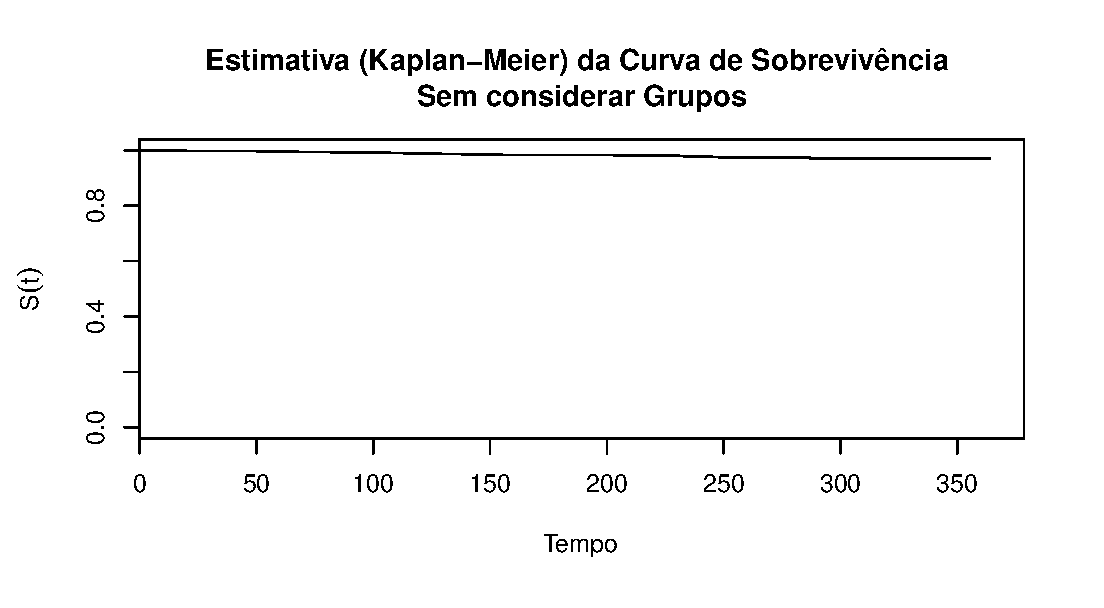
\includegraphics[scale = 0.9]{Rplot01}
    \caption*{\tiny{\textbf{Fonte}: Estudo 320 do \textit{AIDS Clinical Trials Group}} \\  \tiny{\textbf{Nota}:As marcações de falha foram omitidas.}}
\end{figure}

Ao analisar a Curva do Tempo Total em Teste (Curva TTT) na Figura \ref{fig:exp3}, temos fortes evidências quanto à utilização de um Modelo Paramétrico cuja função taxa de falha seja monotonicamente crescente.

\begin{figure}[!ht]
	\centering
    \caption{Curva do Tempo Total sob Teste para a variável tempo}
    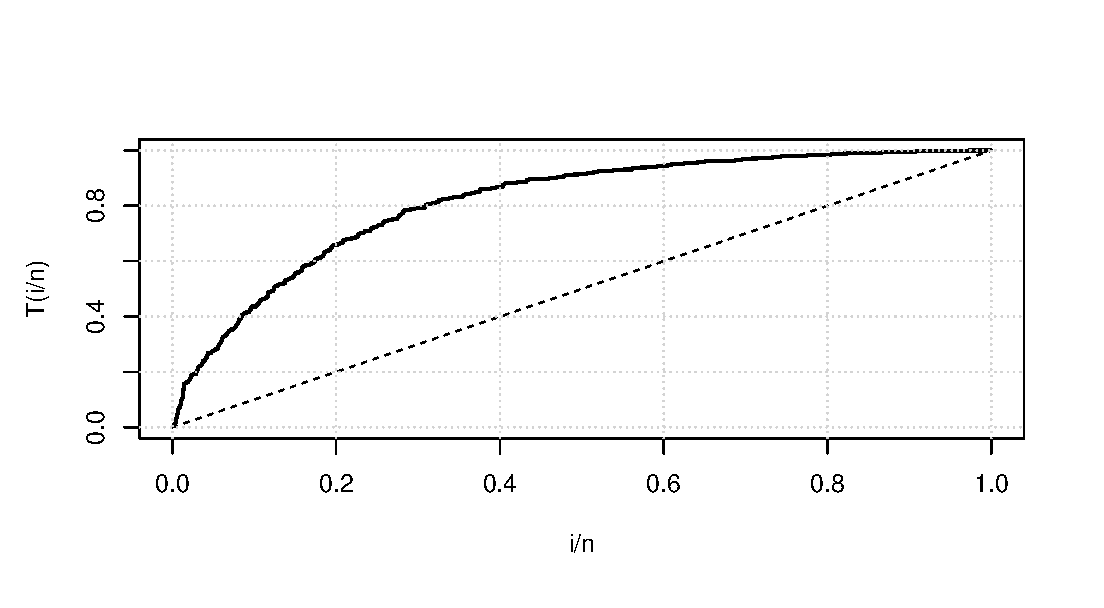
\includegraphics[scale = 0.9]{Rplot02}
    \label{fig:exp3}
\end{figure}

\section{Descrição Resumida das Covariáveis}
A Tabela \ref{tab:expdesccovar} e os gráficos da Figura \ref{fig:expkern} descrevem as covariáveis do estudo. 

\begin{table}[!ht]
	\caption{Descrição das Covariáveis qualitativas, seus níveis e respectivos números de observações}
    \label{tab:expdesccovar}
    \centering
	\begin{tabular}{ccc}
    	\hline
		Covariável & Níveis (\#) &Número de Observações \\\hline
        \multirow{2}{*}{Tratamento} & Controle (0) & 
         577\\
        						\   & Tratamento (1) & 574\\\hline
        \multirow{4}{*}{Grupo de Tratamento} & ZDV + 3TC (1) & 
         576\\
         						\	& ZDV + 3TC + IDV (2) & 572 \\
                                \	& d4T + 3TC (3) & 1 \\
                                \	& d4T + 3TC (4) & 2 \\\hline				\multirow{2}{*}{Sexo} & Masculino (1) & 951 \\
         						\ & Feminino (2) & 200 \\\hline
        \multirow{2}{*}{Estrato CD4} & $\leq 50/mm^3$ (0) & 439 \\
         						\ & $\geq 50/mm^3$ (1) & 712\\\hline
         \multirow{5}{*}{Raça/Etnia} & Branco Não-Hispânico (1) & 596 \\
         						\ & Negro Não-Hispânico (2) & 327\\
                                \ & Hispânico (3) & 203 \\
                                \ & Asiático, Ilhas do Pacífico (4) & 14\\
                                \ & Indo-Americano, Nativo do Alasca (5) & 11 \\\hline	
         \multirow{3}{*}{Utilização de drogas EV} & Nunca (1) & 968 \\
         						\ & Atualmente (2) & 4 \\
                                \ & Previamente (3) & 179 \\\hline
         \multirow{2}{*}{Hemofilia} & Não (0) & 1116 \\
         						\	& Sim (1) & 35 \\\hline
          \multirow{4}{*}{Escore de Karnof} & Cuida de si (70) & 32 \\
          						\ & Normal c/ esforço (80) & 182\\
                                \ & Normal possível (90) & 541 \\
                                \ & Normal (100) & 396\\\hline
                                
         
	\end{tabular}
    \caption*{\tiny{\textbf{Fonte}: Estudo 320 do \textit{AIDS Clinical Trials Group}}} 
\end{table}

\begin{figure}[!ht]
\centering
  \caption{Gráficos de densidade \textit{Kernel} para as covariáveis quantitativas.}
  \begin{tabular}{c}
    \label{fig:expkern}
  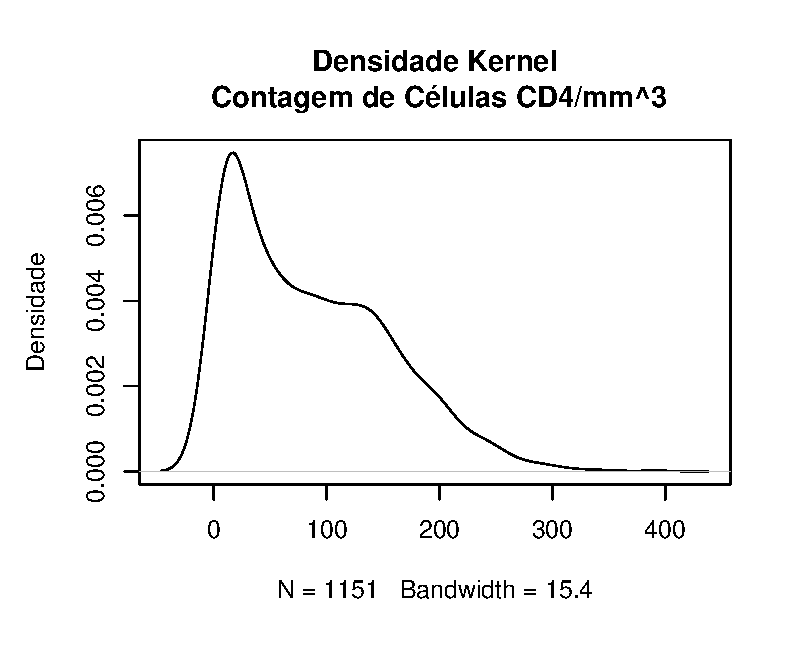
\includegraphics[scale = 0.6]{Rplot11}\\
(a) Covariável contagem de células CD4/$mm^3$ \\
 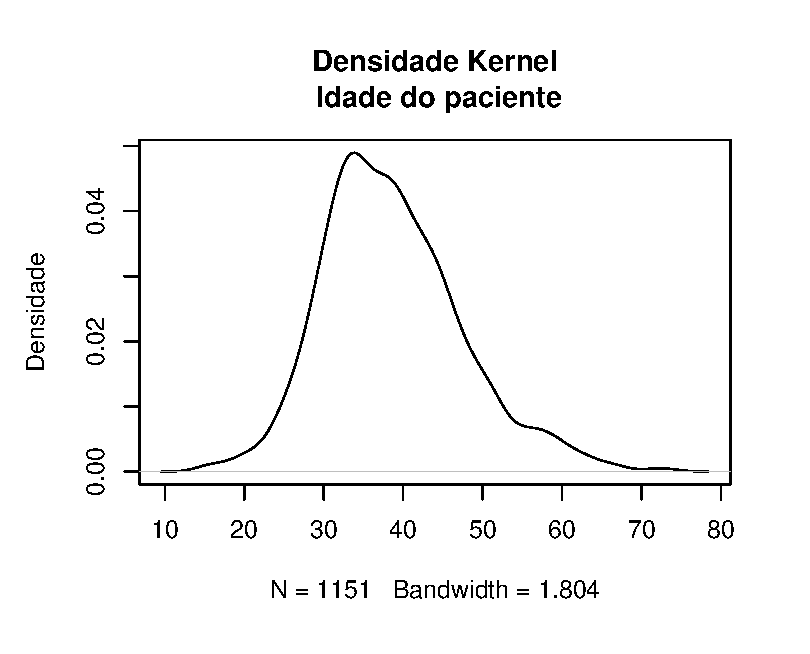
\includegraphics[scale = 0.6]{Rplot12} \\
(b) Covariável idade (anos) do paciente ao início do estudo \\[6pt]
 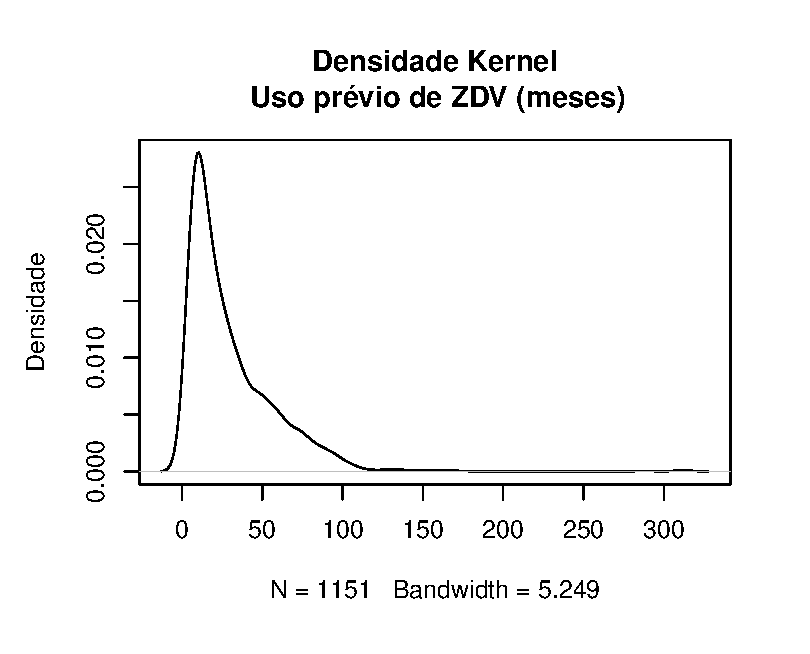
\includegraphics[scale = 0.6]{Rplot13}\\
(c) Covariável uso prévio (meses) de ZDV\\[6pt]
  \end{tabular}
      \caption*{\tiny{\textbf{Fonte}: Estudo 320 do \textit{AIDS Clinical Trials Group}}}
\end{figure}

\section{Avaliação de diferenças das curvas de sobrevivência entre os grupos das covariáveis}

As Figuras \ref{fig:expdif1} e \ref{fig:expdif2} contém tais gráficos utilizando as curvas de sobrevivência estimadas via Método de Kaplan-Meier para as 8 covariáveis qualitativas do estudo e seus respectivos grupos. A inspeção visual é gravemente prejudicada pela natureza do fenômeno em questão: muitas covariáveis tem pouquíssimas observações em certos níveis - e.g. somente 5 indígenas americanos\footnote{Usualmente denominados \textit{native americans} em inglês} participaram do estudo - enquanto para outras covariáveis - e.g. Estrato de contagem de células CD4 - as curvas são tão próximas que a visualização da possível diferença entre elas é gravemente prejudicado.

\begin{figure}[!ht]
  \caption{Estimativas para as curvas de sobrevivência das covariáveis qualitativas.}
  \begin{tabular}{cc}
    \label{fig:expdif1}
  \includegraphics[width=65mm]{Rplot03} &   \includegraphics[width=65mm]{Rplot04} \\
(a) Covariável Tratamento & (b) Covariável Grupo de Tratamento \\[6pt]
 \includegraphics[width=65mm]{Rplot05} &   \includegraphics[width=65mm]{Rplot06} \\
(c) Covariável estrato contagem CD4 & (d) Covariável Sexo \\[6pt]
 \includegraphics[width=65mm]{Rplot07} &   \includegraphics[width=65mm]{Rplot08} \\
(e) Covariável uso de drogas EV & (f) Covariável Hemofilia \\[6pt]
  \end{tabular}
      \caption*{\tiny{Nota:As marcações de falha foram omitidas.}}
\end{figure}

\begin{figure}[!ht]
  \caption{Estimativas para as curvas de sobrevivência das covariáveis qualitativas (continuação).}
  \begin{tabular}{cc}
    \label{fig:expdif2}
  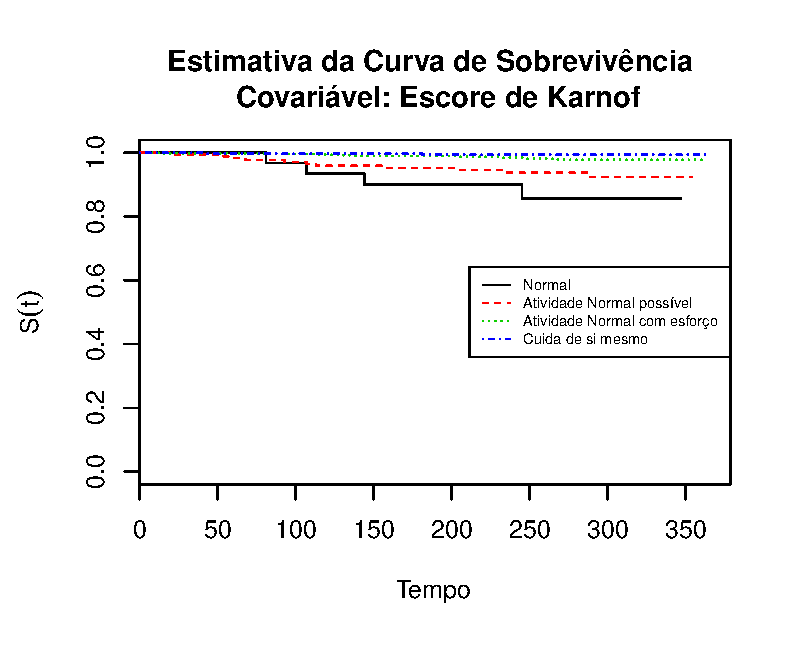
\includegraphics[width=65mm]{Rplot09} &   \includegraphics[width=65mm]{Rplot10} \\
(a) Covariável Escore de Karnoff & (b) Covariável raça/etnia \\[6pt]
  \end{tabular}
        \caption*{\tiny{Nota:As marcações de falha foram omitidas.}}

\end{figure}

A realização de um Teste de Hipóteses para verificar a diferença entre as curvas de sobrevivência faz-se necessária tanto pelo motivo da difícil inspeção visual dos Gráficos das Figuras \ref{fig:expdif1} e \ref{fig:expdif2} quanto pelo fato de tal inspeção ser apenas verificatória, preliminar. A Tabela \ref{tab:expdif1} ilustra quais covariáveis apresentam diferenças estatisticamente significativas a um nível $\alpha = 0,05$ entre as curvas de sobrevivência correspondentes a seus nível utilizando o Teste de Gehan-Wilcoxon implementado na função \texttt{survdiff} do pacote \texttt{survival} do R.

\begin{table}[!ht]
	\caption{Covariáveis que apresentaram diferença significativa entre seus grupos segundo o Teste de Gehan-Wilcoxon}
    \label{tab:expdif1}
    \centering
	\begin{tabular}{ccc}
    	\hline
		Covariável & Níveis &Nível de Significância \\\hline
        \multirow{2}{*}{Tratamento} & Controle (0) & \multirow{2}{*}{0,0443} \\
        						\   & Tratamento (1) \\\hline
         \multirow{2}{*}{Estrato CD4} & $\leq 50/mm^3$ & \multirow{2}{*}{0,00164} \\
         						\ & $\geq 50/mm^3$ & \\\hline
         \multirow{5}{*}{Raça/Etnia} & Branco Não-Hispânico (1) & \multirow{5}{*}{0,0227†} \\
         						\ & Negro Não-Hispânico (2) & \\
                                \ & Hispânico (3) & \\
                                \ & Asiático, Ilhas do Pacífico (4) & \\
                                \ & Indo-Americano, Nativo do Alasca (5) & \\\hline	
         \multirow{3}{*}{Utilização de drogas EV} & Nunca (1) & \multirow{3}{*}{0,0106††} \\
         						\ & Atualmente (2) & \\
                                \ & Previamente (3) & \\\hline
          \multirow{4}{*}{Escore de Karnoff} & Cuida de si (70) & \multirow{4}{*}{$\approx 10^{-7}$} \\
          						\ & Normal c/ esforço (80) & \\
                                \ & Normal possível (90) & \\
                                \ & Normal (100) & \\\hline
                                
         
	\end{tabular}
    \caption*{\textbf{Notas}:\tiny{† baixa contagem nas categorias 4 (14) e 5 (11), teste pouco confiável}\\ 
    \tiny{†† baixa contagem na categoria 2 (4 casos), teste pouco confiável}} 
\end{table}

% ----------------------------------------------------------
% PARTE
% ----------------------------------------------------------
\part{Modelagem}
% ----------------------------------------------------------

\chapter{Escolha do Modelo Semi-paramétrico}

Segundo a Curva do Tempo Total sob Teste em \ref{fig:exp3}, a função de risco tem comportamento monótono crescente, o que sustenta a utilização de um modelo paramétrico Weibull com $\gamma > 1$. Como neste foi considerado um modelo semi-paramétrico para o fenômeno, cabe aqui um breve comentário sobre sua definição. Sob suposição de proporcionalidade dos riscos, i.e. $\frac{h_1(t)}{h_0(t)} = K$ para as respectivas funções de risco dos grupos 0 e 1 (extensível para uma quantidade maior), temos que a função taxa de falha do Modelo de Cox é dada por:

\begin{equation}
\label{eq:modelosp}
h(t|x) = \begin{cases}
h_1(t) = h_0(t)g(\boldsymbol{x'}\boldsymbol{\beta}), & \mbox{se grupo 1} \\
h_0(t), & \mbox{se grupo 0}
\end{cases}
\end{equation}

onde g é uma função não-negativa a ser especificada, $\boldsymbol{x}$ é o vetor p-dimensional de p covariáveis e $\boldsymbol{\beta}$ é o vetor p-dimensional de coeficientes a ser estimado. \cite{kalbfleisch2011statistical} mostraram que a Distribuição Weibull é um caso particular em \ref{eq:modelosp} com $h_0(t) = \frac{\gamma}{\alpha^{\gamma}}t^{\gamma-1}$, então pode ser o caso em que o Modelo Weibull pode ser utilizado ainda que nosso contexto seja semi-paramétrico, como evidenciado, novamente, pela Curva do Tempo Total sob Teste em \ref{fig:exp3}.

A próxima etapa consiste, então, em verificar a suposição de riscos proporcionais para as covariáveis do estudo. Aquelas covariáveis para a qual esta suposição vale podem ser incluídas no Modelo \ref{eq:modelosp}.

\section{Verificação da suposição de Riscos Proporcionais}

Tradicionalmente, esta suposição é avaliada de maneira preliminar inspecionando os gráficos das curvas de sobrevivência estimadas de acordo com os respectivos níveis das covariáveis: espera-se que não haja cruzamento entre elas. Como os Gráficos em \ref{fig:expdif1} e \ref{fig:expdif2} são pouco informativos, faz-se necessário o uso de um teste de hipóteses adequado para avaliar a suposição, seus resultados globais estão na Tabela \ref{tab:thrp}. Estes Testes são baseados na Correlação Linear de Pearson: se a suposição de riscos proporcionais não é violada, a correlação entre os níveis da covariável é aproximadamente nula. Verificamos que a suposição não é violada para as covariáveis \textbf{Tratamento}, \textbf{Raça/Etnia}, \textbf{Utilização de Drogas Endovenosas} e \textbf{Escore de Karnofski}. 

\begin{itemize}
	\item O Teste rejeita a hipótese nula de proporcionalidade para a covariável \textbf{Estrato de Contagem de Células CD4}. Esse resultado é particularmente problemático porque na literatura médica esta covariável tem importante influência no resultado do tratamento contra HIV e infecções oportunistas. No entanto, a covariável tem papel importante especialmente quando é reavaliada periodicamente ao longo do tratamento, não sendo o caso aqui em análise. Pragmaticamente, a contagem CD4 no início do tratamento sugere a propedêutica a ser adotada: grosso modo contagens menores sugerem tratamentos mais \textit{agressivos}. Como aqui a contagem não serviu como ferramenta de estratificação dos pacientes, essa interpretação não vale. Por isso, vamos rejeitar a suposição de riscos proporcionais para esta covariável e não a utilizaremos em nosso modelo.
	\item No entanto, uma estratificação diferente da proposta pela variável original do conjunto de dados pode ser interessante. Ela será considerada na Seção a seguir.
	\item Para o nível 2 - Negros Não-Hispânicos - da covariável \textbf{Raça/Etnia} o teste individual para a proporcionalidade rejeitou a hipótese nula. Aqui novamente há uma consideração a ser feita em consonância com a literatura médica: mais de três décadas de análise de tratamentos contra o HIV e infecções secundárias não encontraram diferenças significativas entre as taxas de sobrevivência de pacientes submetidos a diferentes tratamentos quando avaliados em relação a suas raças/etnias, portanto esta covariável também não será considerada no nosso modelo de regressão.
	\item A covariável \textbf{Uso de Drogas Endovenosas} possui originalmente baixa contagem no nível 3 - Previamente. Como tal informação é sensível e eventualmente pacientes possam se sentir constrangidos e não informar o pesquisador sobre seu real estado, vamos considerar uma dicotomização para a covariável: 0 se o paciente \textbf{nunca} utilizou drogas endovenosas; e 1 se já utilizou ou utiliza presentemente É nessa formulação que a hipótese de proporcionalidade das curvas de risco não é rejeita, então a covariável transformada desta forma será incluída no Modelo.
	\item \cite{hosmer}, como a contagem de pacientes cujo escore de Karnofski é igual a 70 é muito baixa, podemos dicotomizar uma nova variável, \textbf{karnof_70}, que indica quando o paciente teve este escore. Como este é o mais baixo escore numa escala qualitativa que indica o estado do paciente, é razoável considerar que pacientes neste estado têm menos chance de sobreviver. O teste de hipóteses baseado na correlação linear para esta nova covariável (não mostrada em \ref{tab:thrp} não rejeita a hipótese de proporcionalidade entre seus níveis.
	\item Por outro lado, pacientes com escore maior ou igual a 90 tem vida "Normal": com suas atividades laborais mantidas ou reduzidas mas sem grandes prejuízos à independência e auto-manutenção. Desta forma, uma outra covariável dicotomizada, \textbf{karnof_90}, que indica quais pacientes tiveram um escore maior ou igual a este valor. O teste de hipóteses baseado na correlação linear para esta nova covariável (não mostrada em \ref{tab:thrp} não rejeita a hipótese de proporcionalidade entre seus níveis.

\end{itemize}
 
\begin{table}[!ht]
	\caption{Testes baseados na correlação linear de Pearson para avaliar a suposição de riscos proporcionais.}
    \label{tab:thrp}
    \centering
	\begin{tabular}{ccc}
    	\hline
		Covariável & Níveis & Nível de Significância \\\hline
        \multirow{2}{*}{Tratamento} & Controle (0) & \multirow{2}{*}{0,527} \\
        						\   & Tratamento (1) \\\hline
         \multirow{2}{*}{Estrato CD4} & $\leq 50/mm^3$ & \multirow{2}{*}{0,068} \\
         						\ & $\geq 50/mm^3$ & \\\hline
         \multirow{5}{*}{Raça/Etnia} & Branco Não-Hispânico (1) & \multirow{5}{*}{0,1114} \\
         						\ & Negro Não-Hispânico (2) & \\
                                \ & Hispânico (3) & \\
                                \ & Asiático, Ilhas do Pacífico (4) & \\
                                \ & Indo-Americano, Nativo do Alasca (5) & \\\hline	
         \multirow{3}{*}{Utilização de drogas EV} & Nunca (0) & \multirow{3}{*}{0,675} \\
         						\ & Atualmente + Previamente (1) & \\\hline
          \multirow{4}{*}{Escore de Karnoff} & Cuida de si (70) & \multirow{4}{*}{0.713} \\
          						\ & Normal c/ esforço (80) & \\
                                \ & Normal possível (90) & \\
                                \ & Normal (100) & \\\hline
         
	\end{tabular} 
\end{table}



O Gráfico dos Resíduos de Schoenfeld \textit{versus} tempo em \ref{fig:schtime} também é sugerido nesta avaliação como ferramenta preliminar: quando a suposição de riscos proporcionais não é violada a curva de interpolação \textit{lowess} presente no gráfico é aproximadamente constante. Mas a inspeção desses gráficos geralmente é pouco descritiva quando a violação da suposição de proporcionalidade não é gravemente ferida.

\begin{figure}[!ht]
  \caption{Gráficos de Resíduos de Schoenfeld \textit{versus} tempo para as covariáveis qualitativas.}
  \begin{tabular}{cc}
    \label{fig:expdif1}
  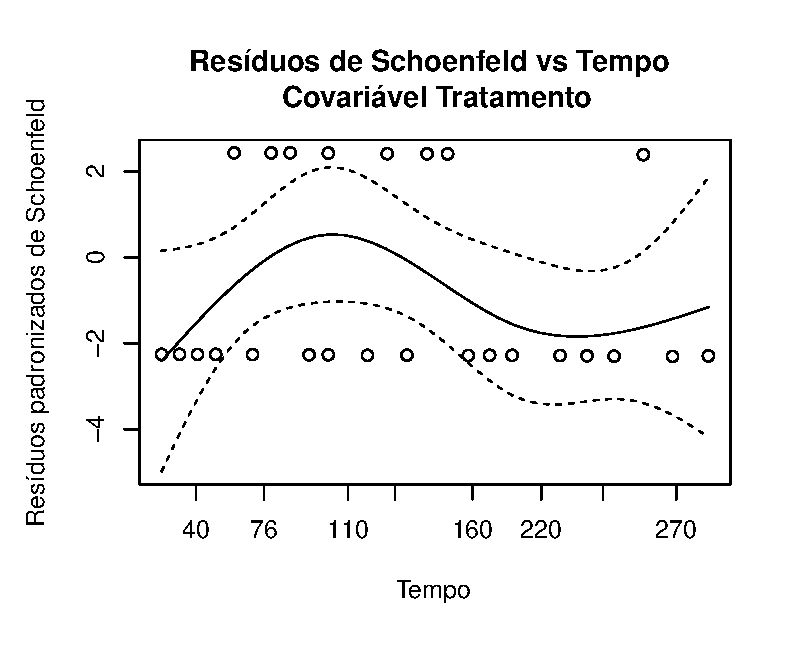
\includegraphics[width=65mm]{Rplot14} &   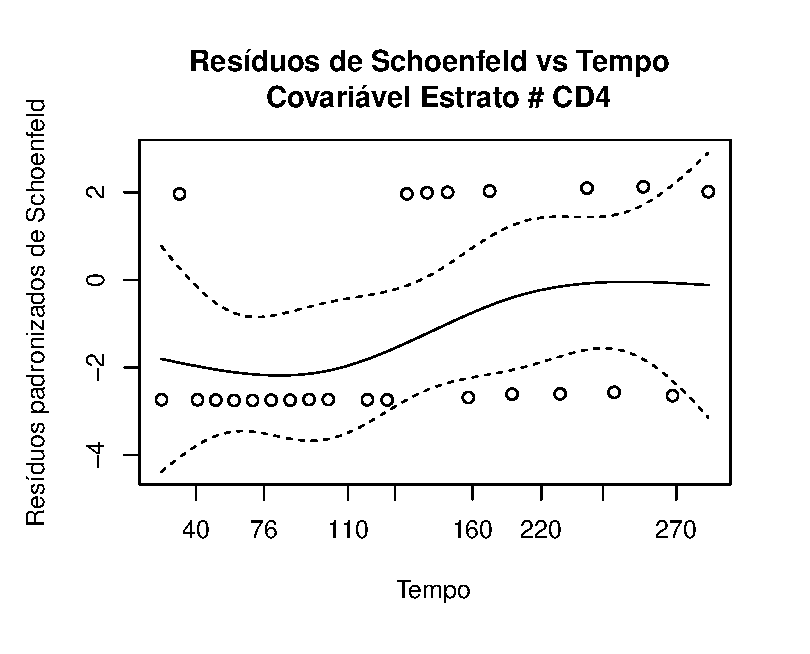
\includegraphics[width=65mm]{Rplot15} \\
(a) Covariável Tratamento & (b) Covariável Estrato CD4 \\[6pt]
 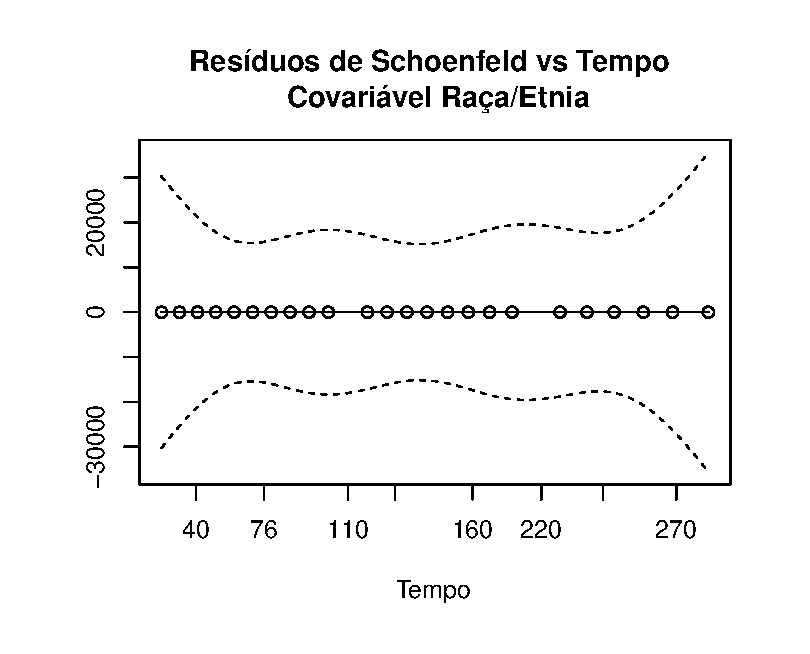
\includegraphics[width=65mm]{Rplot18} &   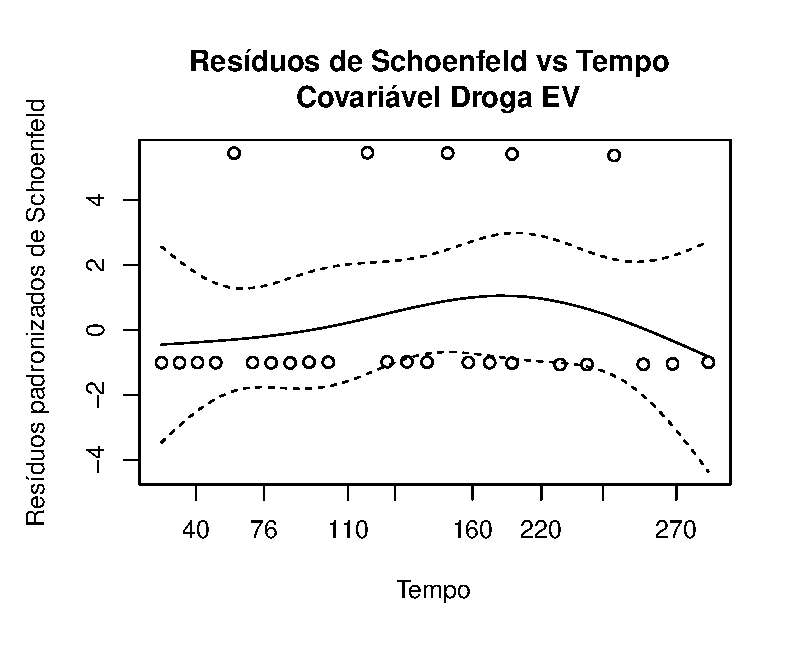
\includegraphics[width=65mm]{Rplot19} \\
(c) Covariável raça/etnia & (d) Covariável Droga EV Transformada \\[6pt]
 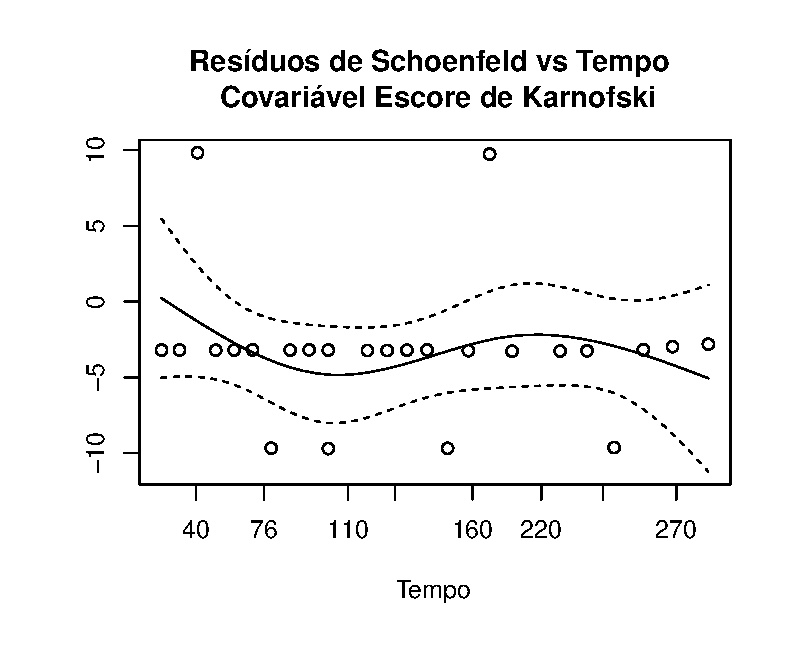
\includegraphics[width=65mm]{Rplot17} &   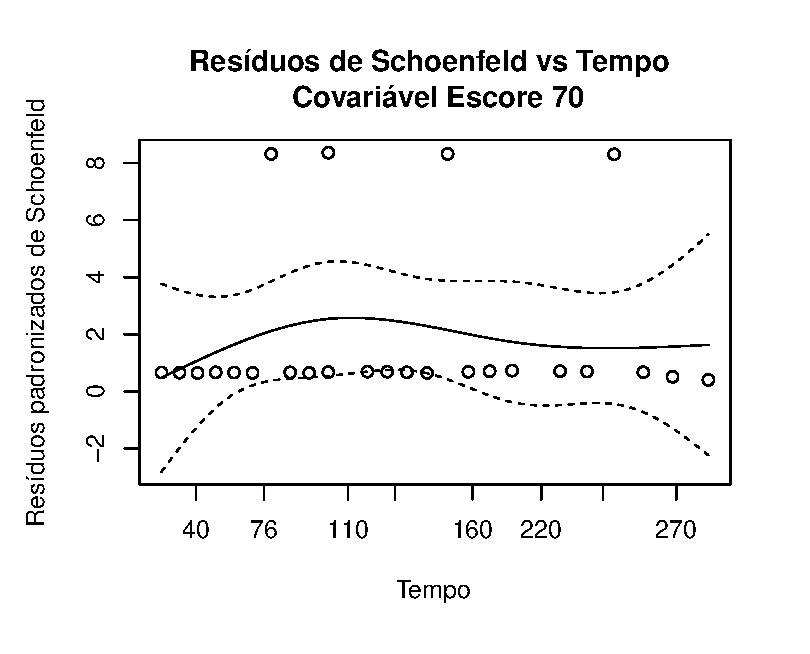
\includegraphics[width=65mm]{Rplot20} \\
(e) Covariável Escore de Karnofski & (f) Covariável Escore Karnofski 70 \\[6pt]
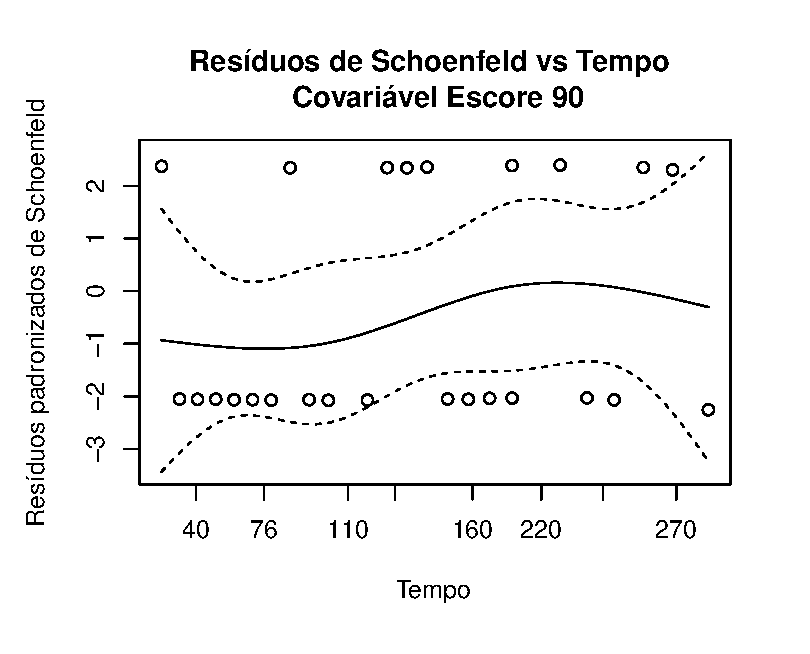
\includegraphics[widht=65mm]{Rplot21} & \\
(f) Covariável Escore Karnofski 90 \\[6pt]
  \end{tabular}
      \caption*{\tiny{Nota:As marcações de falha foram omitidas.}}
\end{figure}


\section{Comparação de Modelos}

Os modelos com suas respectivas covariáveis estão na Tabela \ref{tab:modelos}. A escolha dos modelos deve basear-se em evidências apresentadas pela Análise Exploratória feita em \ref{chap:anexp}, e incluir prioritariamente covariáveis que respeitam a suposição de proporcionalidade exigida pelo modelo.

\begin{table}[!ht]
	\caption{Testes baseados na correlação linear de Pearson para avaliar a suposição de riscos proporcionais.}
    \label{tab:thrp}
    \centering
	\begin{tabular}{ccc}
    	\hline
		Modelos & Covariáveis & Estimativas & Log-Verossimilhança Parcial \\\hline
		1 & Nenhuma & - & $l_1 = -177.3552$ \\\hline
		\multirow{2}{*}{2} & Tratamento & $\beta_1 = -0.8324801$ & \multirow{2}{*}{$l_2 = -175.2726}\\
         
	\end{tabular} 
\end{table}

% ----------------------------------------------------------
% PARTE
% ----------------------------------------------------------
\part{Resultados}
% ----------------------------------------------------------

% ----------------------------------------------------------
% Finaliza a parte no bookmark do PDF
% para que se inicie o bookmark na raiz
% e adiciona espaço de parte no Sumário
% ----------------------------------------------------------
\phantompart

% ---
% Conclusão
% ---
\chapter{Conclusão}
% ---

\lipsum[31-33]

% ----------------------------------------------------------
% ELEMENTOS PÓS-TEXTUAIS
% ----------------------------------------------------------
\postextual
% ----------------------------------------------------------

% ----------------------------------------------------------
% Referências bibliográficas
% ----------------------------------------------------------
\bibliography{abntex2-modelo-references}

% ----------------------------------------------------------
% Glossário
% ----------------------------------------------------------
%
% Consulte o manual da classe abntex2 para orientações sobre o glossário.
%
%\glossary

% ----------------------------------------------------------
% Apêndices
% ----------------------------------------------------------

% ---
% Inicia os apêndices
% ---
\begin{apendicesenv}

% Imprime uma página indicando o início dos apêndices
\partapendices

% ----------------------------------------------------------
\chapter{Quisque libero justo}
% ----------------------------------------------------------

\lipsum[50]

% ----------------------------------------------------------
\chapter{Nullam elementum urna vel imperdiet sodales elit ipsum pharetra ligula
ac pretium ante justo a nulla curabitur tristique arcu eu metus}
% ----------------------------------------------------------
\lipsum[55-57]

\end{apendicesenv}
% ---


% ----------------------------------------------------------
% Anexos
% ----------------------------------------------------------

% ---
% Inicia os anexos
% ---
\begin{anexosenv}

% Imprime uma página indicando o início dos anexos
\partanexos

% ---
\chapter{Morbi ultrices rutrum lorem.}
% ---
\lipsum[30]

% ---
\chapter{Cras non urna sed feugiat cum sociis natoque penatibus et magnis dis
parturient montes nascetur ridiculus mus}
% ---

\lipsum[31]

% ---
\chapter{Fusce facilisis lacinia dui}
% ---

\lipsum[32]

\end{anexosenv}

%---------------------------------------------------------------------
% INDICE REMISSIVO
%---------------------------------------------------------------------
\phantompart
\printindex
%---------------------------------------------------------------------

\end{document}
